%%%%%%%%%%%%%%%%%%%%%%%%%%%%%%%%%%%%%%%%%
% baposter Portrait Poster
% LaTeX Template
% Version 1.0 (15/5/13)
%
% Created by:
% Brian Amberg (baposter@brian-amberg.de)
%
% This template has been downloaded from:
% http://www.LaTeXTemplates.com
%
% License:
% CC BY-NC-SA 3.0 (http://creativecommons.org/licenses/by-nc-sa/3.0/)
%
%%%%%%%%%%%%%%%%%%%%%%%%%%%%%%%%%%%%%%%%%

%----------------------------------------------------------------------------------------
%	PACKAGES AND OTHER DOCUMENT CONFIGURATIONS
%----------------------------------------------------------------------------------------

\documentclass[a0paper,portrait]{baposter}

\usepackage[font=small,labelfont=bf]{caption} % Required for specifying captions to tables and figures
\usepackage{booktabs} % Horizontal rules in tables
\usepackage{relsize} % Used for making text smaller in some places
\usepackage{amsmath}
\usepackage{wrapfig}
\usepackage{graphicx}


\graphicspath{{figures/}} % Directory in which figures are stored

\definecolor{bordercol}{RGB}{40,40,40} % Border color of content boxes
\definecolor{headercol1}{RGB}{186,215,230} % Background color for the header in the content boxes (left side)
\definecolor{headercol2}{RGB}{80,80,80} % Background color for the header in the content boxes (right side)
\definecolor{headerfontcol}{RGB}{0,0,0} % Text color for the header text in the content boxes
\definecolor{boxcolor}{RGB}{255,255,255} % Background color for the content in the content boxes

\begin{document}

\background{ % Set the background to an image (background.pdf)
\begin{tikzpicture}[remember picture,overlay]
\draw (current page.north west)+(-2em,2em) node[anchor=north west]
{
\includegraphics[height=1.1\textheight]{background}};
\end{tikzpicture}
}

\begin{poster}{
grid=false,
borderColor=bordercol, % Border color of content boxes
headerColorOne=headercol1, % Background color for the header in the content boxes (left side)
headerColorTwo=headercol2, % Background color for the header in the content boxes (right side)
headerFontColor=headerfontcol, % Text color for the header text in the content boxes
boxColorOne=boxcolor, % Background color for the content in the content boxes
headershape=roundedright, % Specify the rounded corner in the content box headers
headerfont=\Large\sf\bf, % Font modifiers for the text in the content box headers
textborder=rectangle,
background=user,
headerborder=open, % Change to closed for a line under the content box headers
boxshade=plain
}
{}
%
%----------------------------------------------------------------------------------------
%	TITLE AND AUTHOR NAME
%----------------------------------------------------------------------------------------
%
{\sf\bf Fast Parallel SAME Gibbs Sampling on \\ General Discrete Bayesian Networks} % Poster title
{\vspace{1em}Daniel Seita, Haoyu Chen \& John Canny \\ % Author names
{\smaller seita@berkeley.edu, haoyuchen@berkeley.edu, jfc@cs.berkeley.edu}} % Author email addresses
{
\includegraphics[scale=0.3]{berkeleylog}} % University/lab logo

%----------------------------------------------------------------------------------------
%	INTRODUCTION
%----------------------------------------------------------------------------------------

\headerbox{Introduction}{name=introduction,column=0,row=0}{

A fundamental task in machine learning and related fields is to perform inference on Bayesian networks. Since exact inference takes exponential time, it is common to use an approximate algorithm such as Gibbs sampling, but this can still be intractable for graphical models with just a few hundred binary random variables. In this project, we:
\begin{itemize}
	\item Build a highly optimized Gibbs sampler
	\item Apply SAME to reduce variance
	\item Benchmark our Gibbs sampler on real dataset.
\end{itemize}

}

%----------------------------------------------------------------------------------------
%	MATERIALS AND METHODS
%----------------------------------------------------------------------------------------

\headerbox{Fast Parallel SAME Sampling}{name=methods,column=0,below=introduction}{


SAME (State Augmentation for Marginal Estimation) [1, 2, 3] can be viewed as cooling the posterior parameter distribution and allows annealed search for the MAP parameters, often yielding very high quality (lower loss) estimates.
Given a distribution $P(X,Z\mid \Theta)$, to estimate the most likely $\Theta$ based on the data
$(X,Z)$ using SAME, one would define a new joint $Q$:
\begin{equation*}
Q(X,\Theta,Z^{(1)},\ldots,Z^{(m)}) = \prod_{j=1}^m P(X,\Theta,Z^{(j)})
\end{equation*}
which models $m$ copies of the distribution tied to the same set of parameters $\Theta$. 
%This new distribution $Q$ is proportional to a \emph{power} of the original distribution, so $Q(\Theta \mid X) \propto (P(\Theta \mid X))^m$. Thus, it has the same optima, including the global optimum, but its peaks are sharpened.

\begin{wrapfigure}{l}{0.5\textwidth}
\vspace{-20pt}
  \begin{center}
    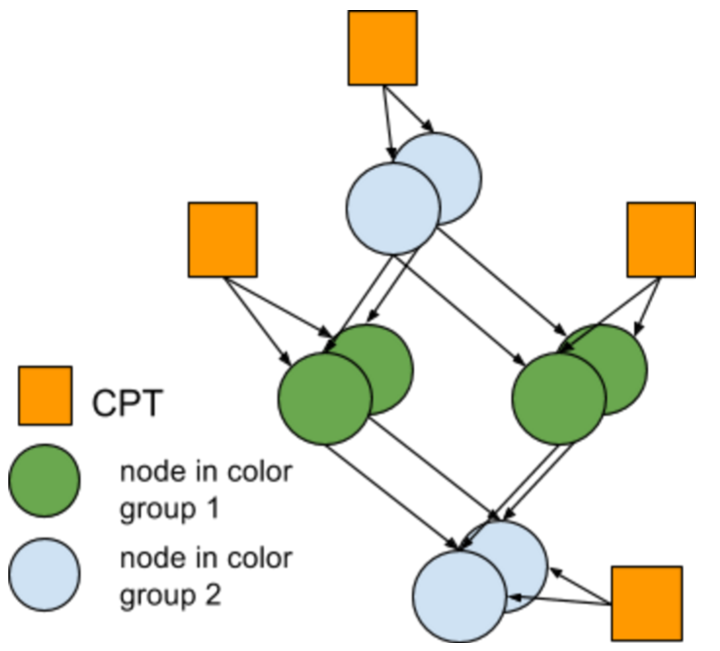
\includegraphics[width=0.5\textwidth]{chy.png}
  \end{center}
  \caption{Gibbs sampler framework (m=2)}
\end{wrapfigure} 
In order to parallel the sampling, we apply graph coloring to the moralized graph of the original network, and within each color group, sample all the variables in parallel. Left figure shows a simple example of three color groups with m=2.



}

%----------------------------------------------------------------------------------------
%	CONCLUSION
%----------------------------------------------------------------------------------------

\headerbox{Conclusion}{name=conclusion,column=0,below=methods}{

We conclude that our Gibbs sampler is much faster than the state of the art (JAGS) in Gibbs sampling and can be applied to data with hundreds of variables. We also argue that SAME is beneficial
for Gibbs sampling, and that it should be the go-to method for researchers who wish to perform inference on (discrete) Bayesian networks. Future work will explore the application of our sampler to a wider class of real-world datasets.
}

%----------------------------------------------------------------------------------------
%	REFERENCES
%----------------------------------------------------------------------------------------

\headerbox{References}{name=references,column=0,below=conclusion}{

\footnotesize % Reduce the font size in this block 
[1] A. Doucet, S. Godsill, and C. Robert. Marginal maximum a posteriori estimation using markov chain monte carlo. Statistics and Computing, 12:77-84, 2002.

[2] C. Robert, A. Doucet, and S. Godsill. Marginal MAP estimation using markov chain monte-carlo. In IEEE Int. Conf. on Acoustics, Speech and Signal Processing, volume 3, pages 1753-1756. IEEE, 1999.

[3] Z. Huasha, J. Biye, and C. John. Same but different: Fast and high quality gibbs parameter estimation. In Proceedings of the 21th ACM SIGKDD International Conference on Knowledge Discovery and Data Mining, KDD '15, pages 1495-1502, NY, USA, 2015. ACM
%\renewcommand{\section}[2]{\vskip 0.05em} 
%\nocite{*} % Insert publications even if they are not cited in the poster

%\bibliographystyle{unsrt}
%\bibliography{sample} % Use sample.bib as the bibliography file
}

%----------------------------------------------------------------------------------------
%	ACKNOWLEDGEMENTS
%----------------------------------------------------------------------------------------

%\headerbox{Acknowledgements}{name=acknowledgements,column=0,below=references, above=bottom}{

%\smaller % Reduce the font size in this block

%} 

%----------------------------------------------------------------------------------------
%	RESULTS 1
%----------------------------------------------------------------------------------------

\headerbox{Implementation}{name=results1,span=2,column=1,row=0}{ % To reduce this block to 1 column width, remove 'span=2'


\begin{wrapfigure}{l}{0.55\textwidth}
  \begin{center}
    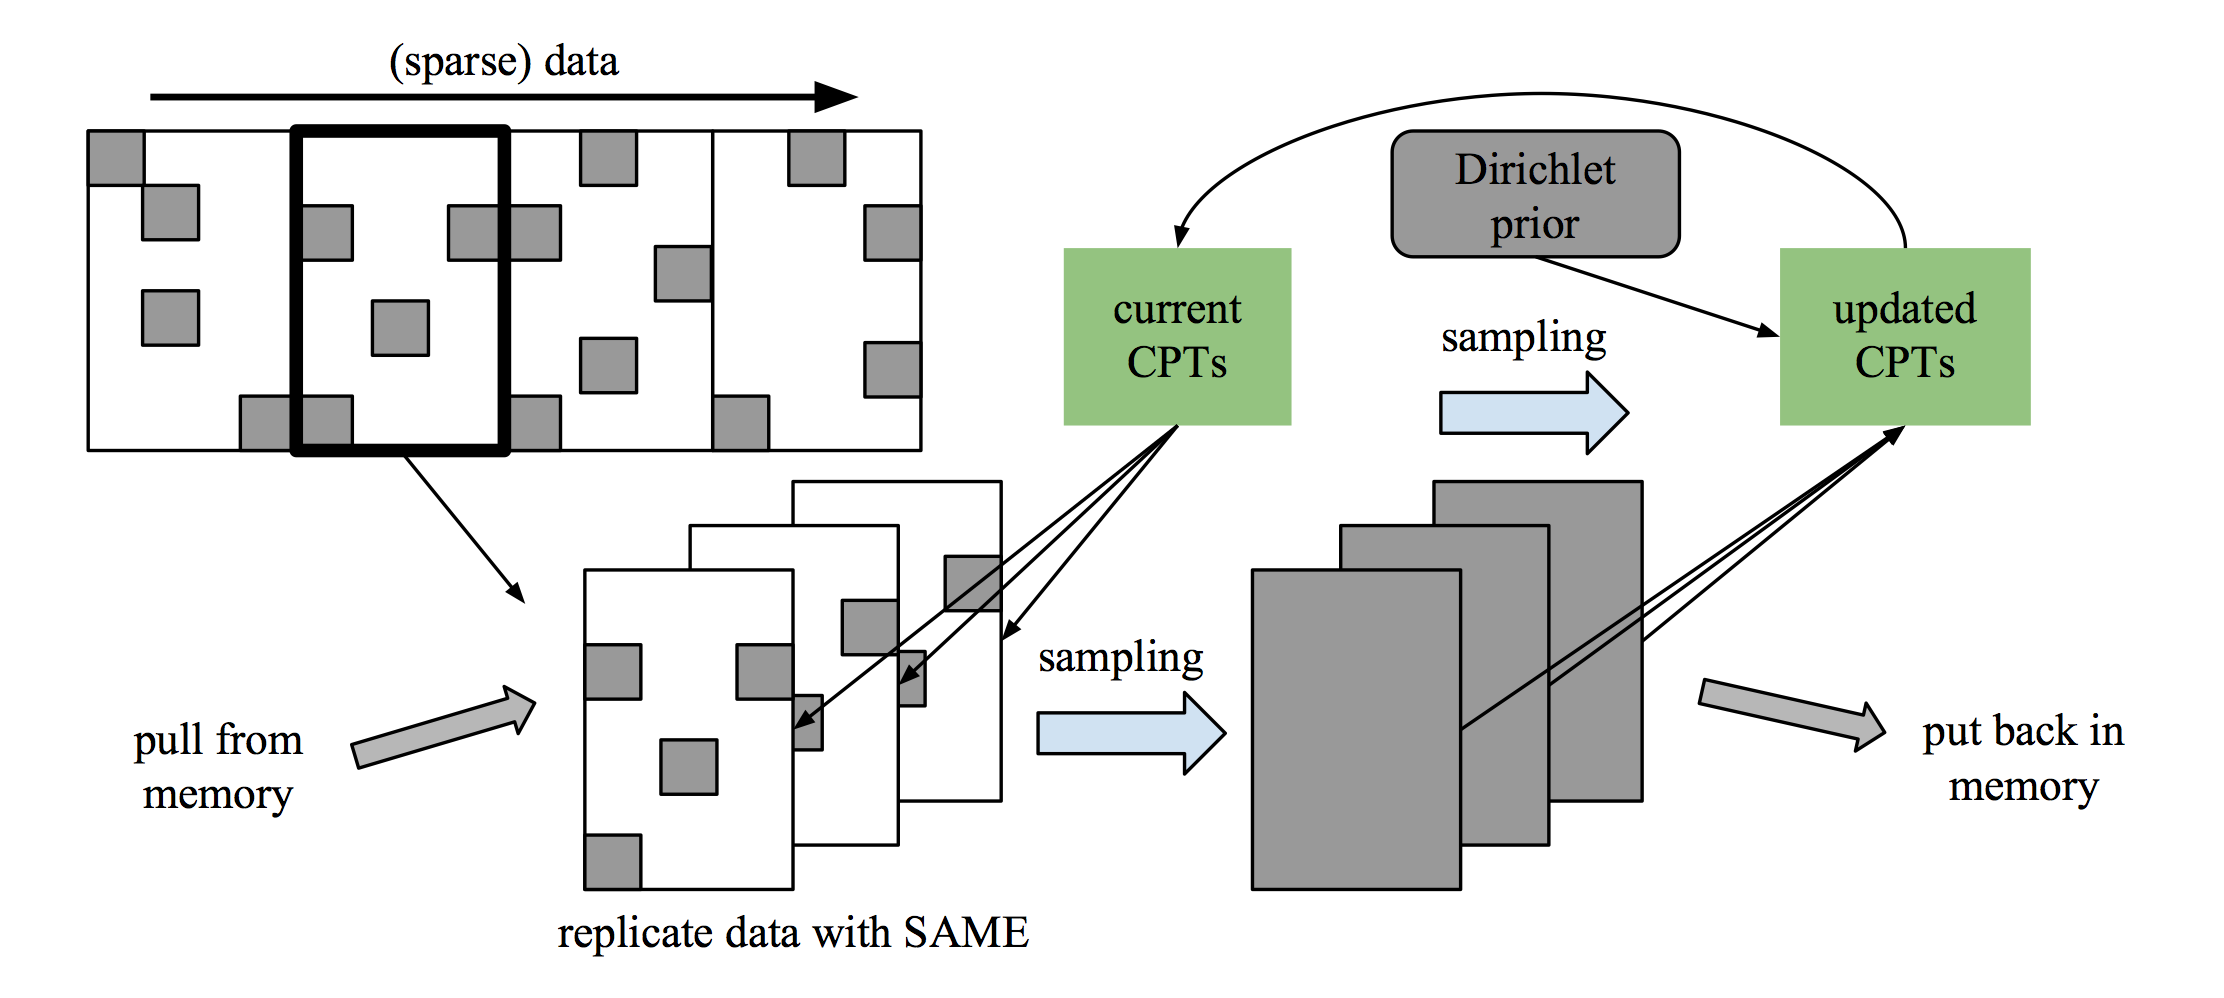
\includegraphics[width=0.5\textwidth]{fig_BIDMach_final}
  \end{center}
  \caption{Gibbs sampler framework}
\end{wrapfigure}
Our Gibbs sampler is implemented and integrated as part of the open-source BIDMach library for machine learning.  Figure 2 shows a visualization of how it works on real data. Our sampler expects a (usually sparse) data matrix, with rows representing variables and columns representing cases. BIDMach divides data into same-sized ``mini-batches'' and iterates through them to update parameters. Going through all mini-batches is one full pass over the data. 

%\begin{center}
%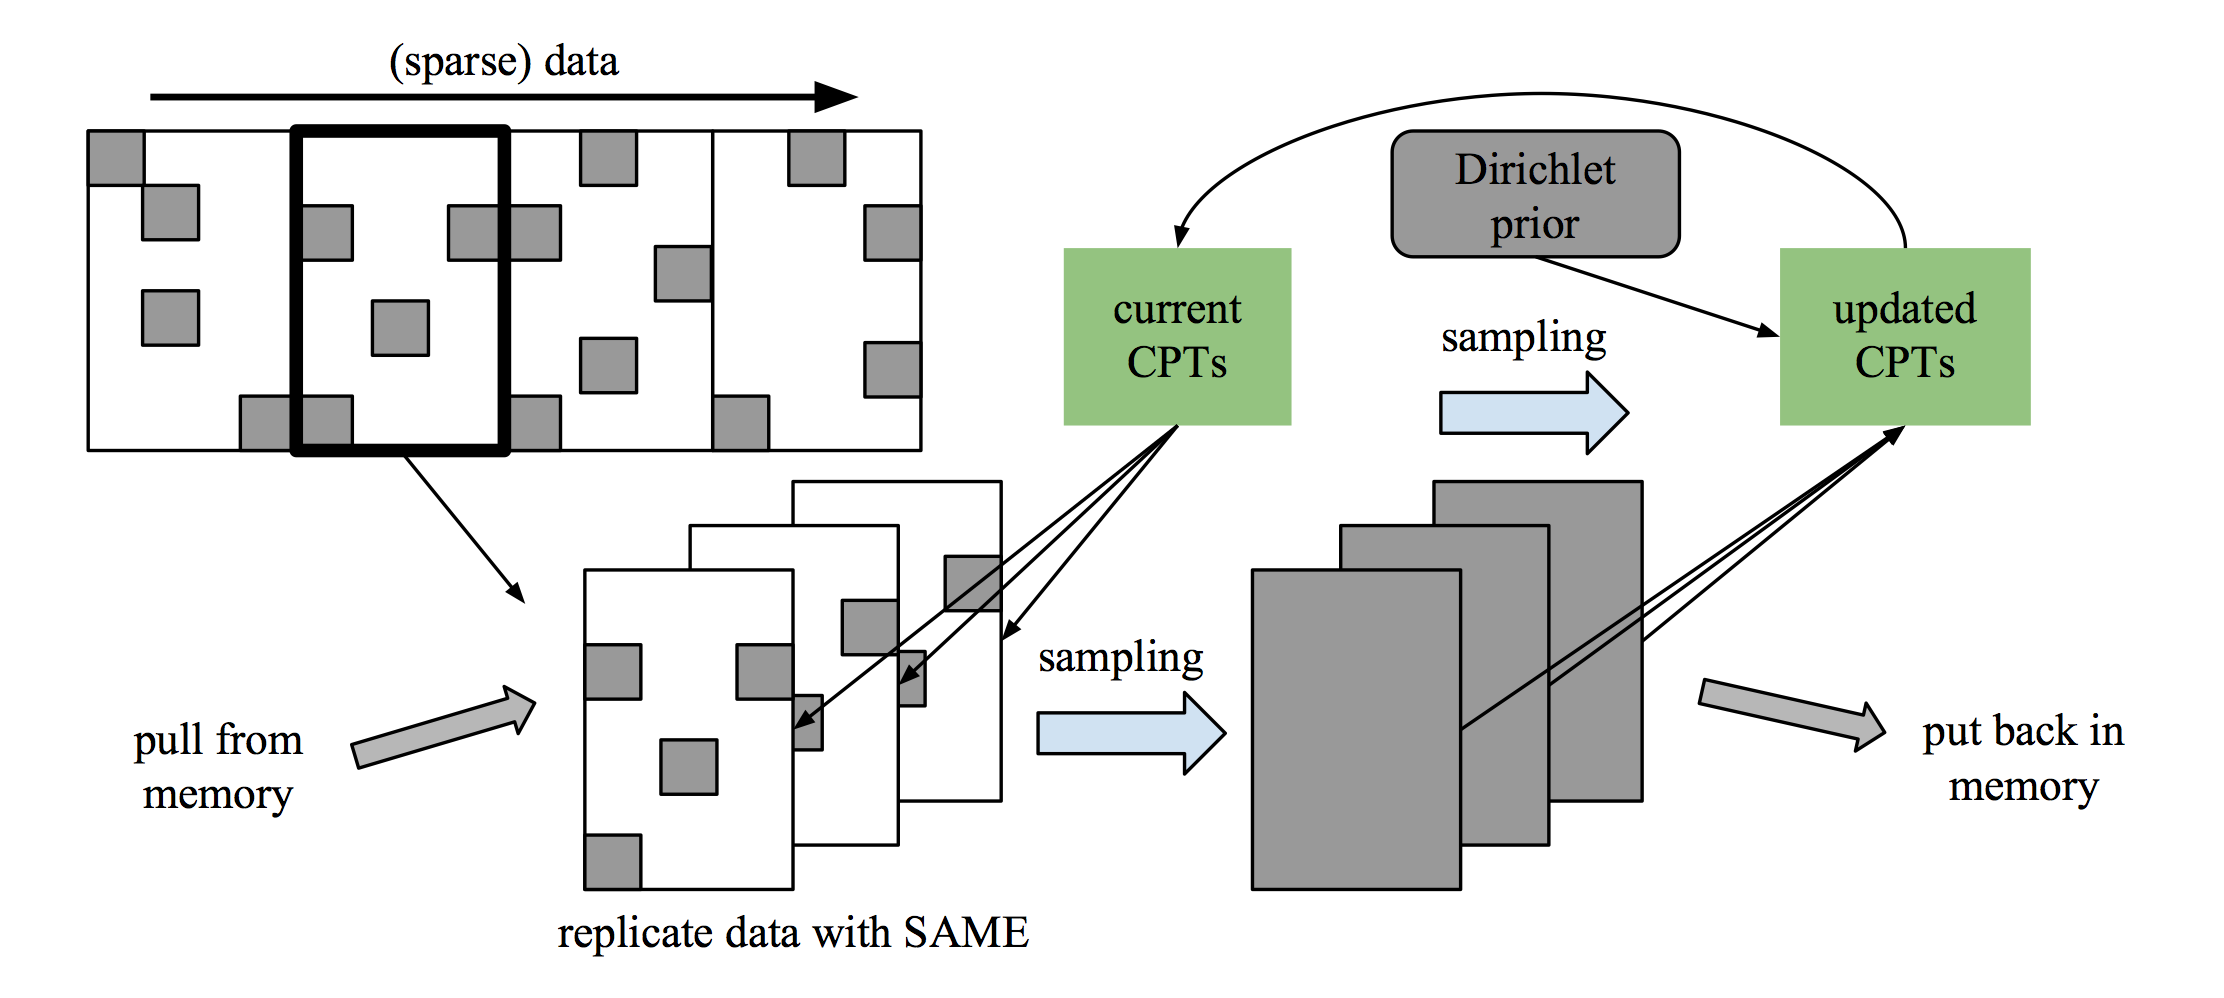
\includegraphics[width=0.60\linewidth]{fig_BIDMach_final}
%\captionof{figure}{Gibbs sampler framework}
%\end{center}

%------------------------------------------------

%\begin{center}
%\begin{tabular}{l l l}
%\toprule
%\textbf{Treatments} & \textbf{Response 1} & \textbf{Response 2}\\
%\midrule
%Treatment 1 & 0.0003262 & 0.562 \\
%Treatment 2 & 0.0015681 & 0.910 \\
%Treatment 3 & 0.0009271 & 0.296 \\
%\bottomrule
%\end{tabular}
%\captionof{table}{Table caption}
%\end{center}
}

%----------------------------------------------------------------------------------------
%	RESULTS 2
%----------------------------------------------------------------------------------------

\headerbox{Experiments}{name=results2,span=2,column=1,below=results1,above=bottom}{ % To reduce this block to 1 column width, remove 'span=2'

We benchmark our code on a nation-wide examination dataset, which contains the assessment (correct or not) of student responses to questions. There were 4367 students and 319 questions. Each question is considered an ``observed'' node in the Bayesian network. We only know 2.2\% of the data. We call the student responses data ``MOOC'' data. We compare our sampler with JAGS.

%------------------------------------------------

\begin{center}
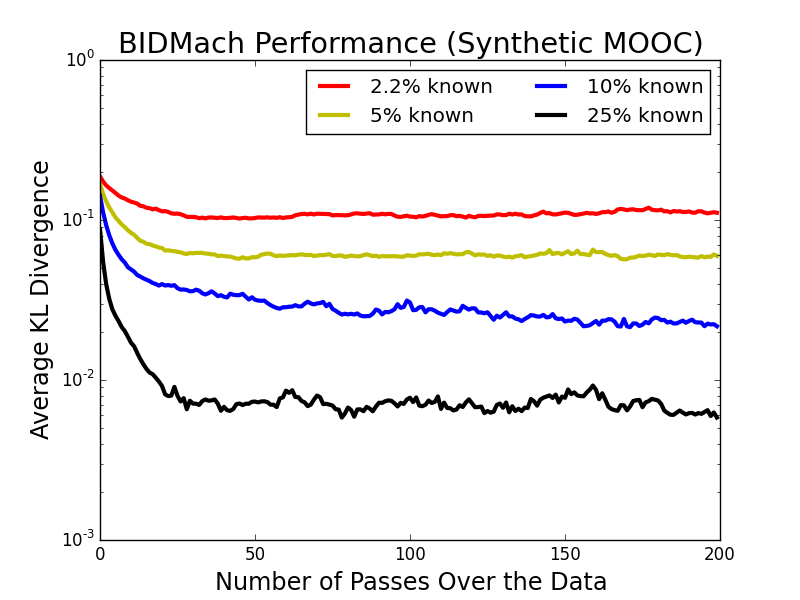
\includegraphics[width=0.45\linewidth]{fig_diff_sparsity_bidmach.png}
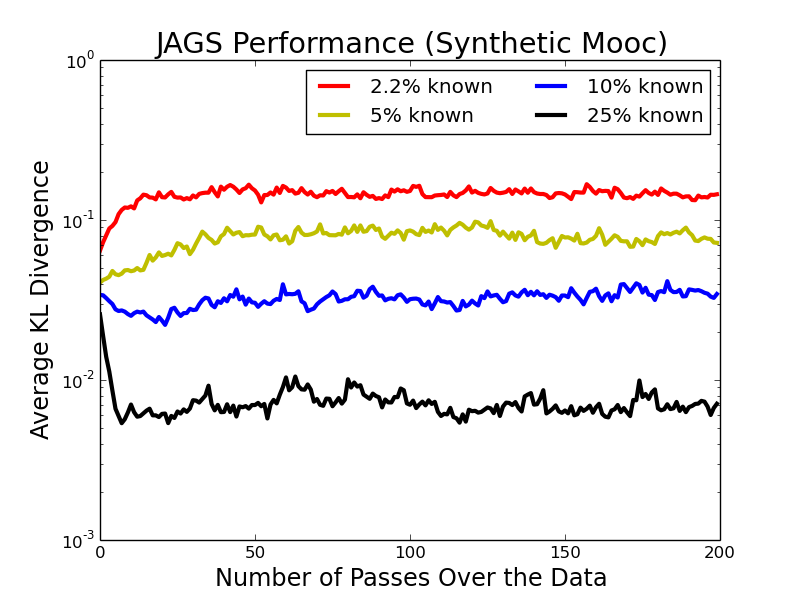
\includegraphics[width=0.45\linewidth]{fig_diff_sparsity_jags.png}
\captionof{figure}{The $KL_{\rm avg}$ from BIDMach. (left); The $KL_{\rm avg}$ from JAGS.(right)}
\end{center}

%------------------------------------------------


\begin{center}
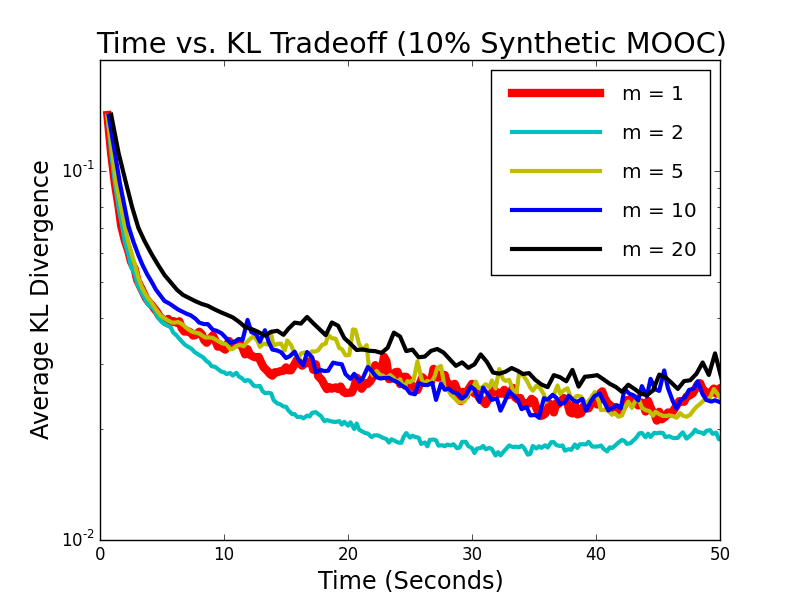
\includegraphics[width=0.45\linewidth]{fig_kltime_tradeoff_mooc.png}
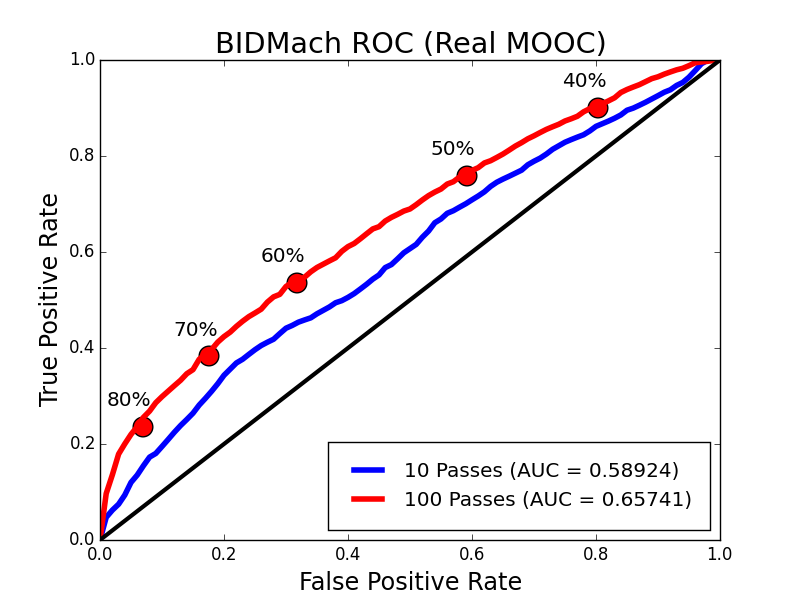
\includegraphics[width=0.45\linewidth]{fig_bidmach_real_mooc_roc_curve_v2.png}
\captionof{figure}{The $KL_{\rm avg}$ vs. runtime for BIDMach. (left); Prediction accuracy of BIDMach(right)}
\end{center}

%------------------------------------------------

%\begin{center}
%
\includegraphics[width=0.6\linewidth]{placeholder}
%\captionof{figure}{Figure caption}
%\end{center}

%------------------------------------------------

In order to show the performance of our sampler in the limit, we replicate the data to increase its size. Table 1 records the runtime (CPU) per iteration for both BIDMach and JAGS, which reveals that our sampler has much shorter runtime than JAGS even without using GPU. 

\begin{center}
\begin{tabular}{ |c|c|c|c|c|c|c| } 
\hline
                  & 1x    & 2x    & 5x    & 10x   & 20x   & 40x   \\
\hline \hline
BIDMach Time(sec)/Iter & 0.182 & 0.375 & 0.931 & 1.792 & 3.501 & 7.181 \\ 
JAGS Time(sec)/Iter    & 4.876 & 13.745 & 29.150 & 94.075 & 171.545 & OOM \\
\hline
\end{tabular}
\captionof{table}{BIDMach (CPU) vs. JAGS Runtime on (Replicated) Real Data}
\end{center}

Table 2 records the BIDMach runtime (GPU) and GigaFlops, which indicates the time and gflops tradeoff.

\begin{center}
\begin{tabular}{ |c|c|c|c|c|c|c|c| } 
\hline
               & $m=1$ & $m=5$ & $m=10$ & $m=20$ & $m=30$ & $m=40$ & $m=50$  \\
\hline \hline
GigaFlops (K)  & 2.38  & 6.98  & 9.08   & 11.00  & 11.70  & 12.27  & 12.35   \\ 
Time/Iter (K)  & 0.307 & 0.523 & 0.804  & 1.328  & 1.872  & 2.380  & 2.957   \\
\hline 
GigaFlops (RM) & 1.65  & 4.58  & 7.08   & 9.69   & 10.92  & 11.62  & 12.02   \\ 
Time/Iter (RM) & 0.666 & 1.192 & 1.541  & 2.252  & 2.998  & 3.753  & 4.536   \\
\hline
\end{tabular}
\captionof{table}{BIDMach (GPU) Runtime vs. GigaFlops on Large Data}
\end{center}

}

%----------------------------------------------------------------------------------------

\end{poster}

\end{document}